\documentclass[]{report}

% Define page
\usepackage[top=1in, bottom=1in, left=1.5in, right=1.5in]{geometry}
\linespread{1.1}

% For math
\usepackage{amsmath,amsthm,amssymb}
\usepackage{bm,url}

% For figures
\usepackage{graphicx,subfigure,psfrag}

\usepackage{natbib}

% Definitions
\newcommand{\elastix}{\texttt{elastix}}
\newcommand{\transformix}{\texttt{transformix}}
\newcommand{\vx}{\bm{x}}
\newcommand{\vu}{\bm{u}}
\newcommand{\vux}{\bm{u}(\bm{x})}
\newcommand{\vmu}{\bm{\mu}}
\newcommand{\vT}{\bm{T}}
\newcommand{\vTm}{\bm{T}_{\vmu}}
\newcommand{\vTmx}{\bm{T}_{\vmu}(\bm{x})}
\newcommand{\CC}{\mathcal{C}}
\newcommand{\NN}{\mathcal{N}}
\newcommand{\Sim}{\mathcal{S}}
\newcommand{\Pen}{\mathcal{P}}

% see page474 latex manual:
\newcommand\relphantom[1]{\mathrel{\phantom{#1}}}

%%%%%%%%%%%%%%%%%%%%%%%%%%%%%%%%%%%%%%%%%%%%%%%%%%%%%%%%%%%%%%%%%%%%%%%%%%%%%%%%%%%%%%%%%%%%

\begin{document}

\title{
\includegraphics[width=8cm]{images/elastixLogo.eps}\\\vspace{1cm}the manual\vspace{1cm}}
\author{Stefan Klein and Marius Staring}
%\date{}
\maketitle

\setcounter{page}{1} \pagenumbering{roman} \tableofcontents
%\newpage
%\listoffigures
%\newpage
%\listoftables
\newpage
\pagenumbering{arabic} \setcounter{page}{1}

%%%%%%%%%%%%%%%%%%%%%%%%%%%%%%%%%%%%%%%%%%%%%%%%%%%%%%%%%%%%%%%%%%%%%%%%%%%%%%%%%%%%%%%%%%%%
% main text

\chapter{Introduction}\label{chp:Introduction}

This manual describes a software package for image registration:
\elastix. The software consists of a collection of algorithms that
are commonly used to solve medical image registration problems. A
large part of the code is based on the Insight Toolkit (ITK). The
modular design of \elastix\ allows the user to quickly test and
compare different registration methods for his/her specific
application. The command-line interface simplifies the processing
of large amounts of data sets, using scripting.

Chapter~\ref{chp:Registration} discusses some general theory of
image registration. Also, the different components of which a
registration method consists are treated. In
Chapter~\ref{chp:elastix}, \elastix\ is described and its usage is
explained. Chapter~\ref{chp:transformix} is dedicated to
\transformix, a program accompanying \elastix. A tutorial is given
in Chapter~\ref{chp:Tutorial}, including many recommendations
based on the authors' own experiences. Chapter~\ref{chp:develop}
provides more details about the source code and explains how to
create extensions of \elastix.

\section{Quick start}

\begin{itemize}
\item Download \elastix\ from
\url{www.isi.uu.nl/Elastix/download.php}.

\item Read some basics about the program at
\url{www.isi.uu.nl/Elastix/about.php} and in this manual.

\item Try the example of usage. It can be found in the \emph{About}
section of the website. If you don't get the example running at your
computer take a look at the FAQ in the general section:
\begin{quote}
\url{www.isi.uu.nl/Elastix/FAQ.php}
\end{quote}

\item Read the complete manual if you are the type of person that
first wants to know.

\item Get started with your own application. If you need more
information at this point you can now start reading the manual. You
can find more information on tuning the parameters in Chapter
\ref{chp:Tutorial}. A list of all available parameters can be found
at \url{www.isi.uu.nl/Elastix/doxygen/pages.html}.

\item When you are stuck, don't miss the tutorial in Chapter
\ref{chp:Tutorial} of this manual. Also, take a look at the FAQ again
for some common problems.

\item When you are still stuck, consult your local registration guru.

\item When you are really stuck you can mail the developers at
\url{elastix@isi.uu.nl}.
\end{itemize}


%%%%%%%%%%%%%%%%%%%%%%%%%%%%%%%%%%%%%%%%%%%%%%%%%%%%%%%%%%%%%%%%%%%%%%%%%%%%%%%%%%%%%%%%%%%%

\chapter{Image registration}\label{chp:Registration}

Image registration is an important tool in the field of medical
imaging. In many clinical situations several images of a patient
are made in order to analyse the patient�s situation. These images
are acquired with, for example, X-ray scanners, Magnetic Resonance
Imaging (MRI) scanners, Computed Tomography (CT) scanners, and
Ultrasound scanners, which provide knowledge about the anatomy of
the subject. Combination of patient data, mono- or multi-modal,
often yields additional clinical information not apparent in the
separate images. For this purpose, the spatial relation between
the images has to be found. Image registration is the task of
finding a spatial one-to-one mapping from voxels in one image to
voxels in the other image, see Figure \ref{fig:concept}. Good
reviews on the subject are given in
\citet{HillEA01,LesterEA99,MaintzEA98}.

The following section introduces the mathematical formulation of
the registration process and gives an overview of the components
of which a general registration method consists. After that, in
Sections~\ref{sec:comp:metric}-\ref{sec:comp:multiresolution},
each component is discussed in more detail.

\section{Registration framework}\label{sec:framework}

\begin{figure}
\centering
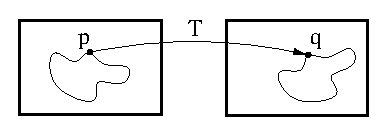
\includegraphics[width=8cm]{images/ImageRegistrationConcept.eps}
\caption{Image registration is the task of finding a spatial
transformation mapping one image to another. Adopted from
\citet{ITKSoftwareGuideSecondEdition}.} \label{fig:concept}
\end{figure}

Two images are involved in the registration process. One image,
the \emph{moving image} $I_M(\vx)$, is deformed to fit the other
image, the \emph{fixed image} $I_F(\vx)$. Registration is the
problem of finding a \emph{displacement} $\vux$ that makes
$I_M(\vx + \vux)$ spatially aligned to $I_F(\vx)$. An equivalent
formulation is to say that registration is the problem of finding
a \emph{transformation} $\vT(\vx) = \vx + \vux $ that makes
$I_M(\vT(\vx))$ spatially aligned to $I_F(\vx)$. The quality of
alignment is defined by a distance or similarity measure $\Sim$,
such as the sum of squared differences (SSD), the correlation
ratio, or the mutual information (MI) measure. Because this
problem is ill-posed, a regularisation or penalty term $\Pen$ is
often introduced that constrains $\vT$.

Commonly, the registration problem is formulated as an optimisation
problem in which the cost function $\mathcal{C}$ is minimised w.r.t.
$\vT$:
\begin{align}
\hat \vT &= \arg \min_{\vT} \CC (\vT; I_F,I_M), \qquad \text{with} \label{eq:registration1}\\
\CC(\vT; I_F,I_M) &= -\Sim(\vT; I_F,I_M) + \gamma
\Pen(\vT),\label{eq:registration2}
\end{align}
where $\gamma$ weighs similarity against regularity. To solve the
above minimisation problem, there are basically two approaches:
parametric and nonparametric. The reader is referred to
\cite{Fis04:Unified} for an overview on nonparametric methods.
Nonparametric methods are further not discussed in this manual.
The \elastix\ software is based on the parametric approach. In
parametric methods, the number of possible transformations is
limited by introducing a parameterisation (model) of the
transformation. The original optimisation problem becomes thus:
\begin{align}
\hat\vTm &= \arg \min_{\vTm}
 \CC(\vTm ; I_F,I_M), \label{eq:towardsparametric}
\end{align}
where the subscript $\vmu$ indicates that the transform has been
parameterised. The vector $\vmu$ contains the values of the
``transformation parameters''. For example, when the
transformation is modelled as a 2D rigid transformation, the
parameter vector $\vmu$ contains one rotation angle and the
translations in $x$ and $y$ direction. We may write Equation
(\ref{eq:towardsparametric}) also as:
\begin{align}
\hat\vmu &= \arg \min_{\vmu} \CC(\vmu; I_F,I_M).
\label{eq:parametric}
\end{align}
From this equation it becomes clear that the original problem
(\ref{eq:registration1}) has been simplified. Instead of
optimising over a ``space of functions $\vT$'', we now optimise
over the three elements of $\vmu$. Examples of other
transformation models are given in
Section~\ref{sec:comp:transform}.

\begin{figure}
\centering
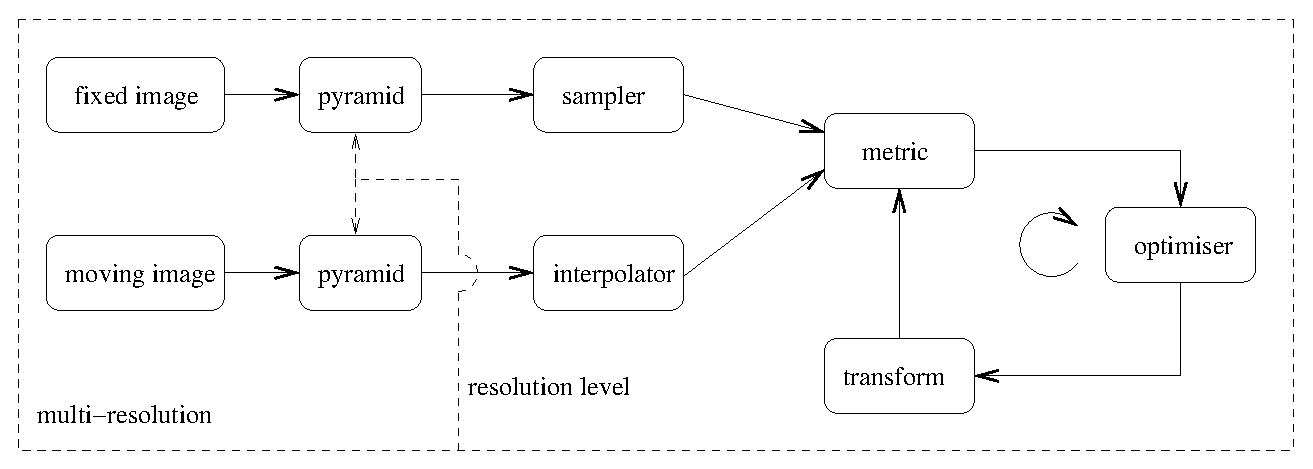
\includegraphics[width=\textwidth]{images/registrationcomponents.eps}
\caption{The basic registration components.}
\label{fig:registrationcomponents}
\end{figure}
Figure~\ref{fig:registrationcomponents} shows the general
components of a parametric registration algorithm in a block
scheme. The scheme is a slightly extended version of the scheme
introduced in \cite{ITKSoftwareGuideSecondEdition}. Several
components can be recognised from Equations
(\ref{eq:registration1})-(\ref{eq:parametric}); some will be
introduced later. First of all, we have the images. The concept of
an image needs to be defined. This is done in
Section~\ref{sec:comp:image}. Then we have the cost function
$\CC$, or ``metric'', which defines the quality of alignment. As
mentioned earlier, the cost function consists of a similarity
measure $\Sim$ and a regularisation term $\Pen$. The
regularisation term $\Pen$ is not discussed in this manual, since
it is often not required in the parametric registration approach.
The similarity measure $\Sim$ is discussed in
Section~\ref{sec:comp:metric}. The definition of the similarity
measure introduces the sampler component, which is treated in
Section~\ref{sec:comp:sampler}. Some examples of transformation
models $\vT_{\vmu}$ are given in Section~\ref{sec:comp:transform}.
The optimisation procedure to actually solve the problem
(\ref{eq:parametric}) is explained in Section
\ref{sec:comp:optimiser}. During the optimisation, the value
$I_M(\vT_{\vmu}(\vx))$ is evaluated at non-voxel positions, for
which intensity interpolation is needed. Choices for the
interpolator are described in Section \ref{sec:comp:interpolator}.
Another thing, not immediately clear from Equations
(\ref{eq:registration1})-(\ref{eq:parametric}), is the use of
multi-resolution strategies to speed-up registration, and to make
it more robust, see Section \ref{sec:comp:multiresolution}.

\section{Images}\label{sec:comp:image}

Since image registration is all about images, we have to be
careful with what is meant by an image. We adopt the notion of an
image from the Insight Toolkit \citep[p.
40]{ITKSoftwareGuideSecondEdition}:

\begin{quote}
Additional information about the images is considered mandatory.
In particular the information associated with the physical spacing
between pixels and the position of the image in space with respect
to some world coordinate system are extremely important. Image
origin and spacing are fundamental to many applications.
Registration, for example, is performed in physical coordinates.
Improperly defined spacing and origins will result in inconsistent
results in such processes. Medical images with no spatial
information should not be used for medical diagnosis, image
analysis, feature extraction, assisted radiation therapy or image
guided surgery. In other words, medical images lacking spatial
information are not only useless but also hazardous.

Figure \ref{fig:image} illustrates the main geometrical concepts
associated with the itk::Image. In this figure, circles are used
to represent the centre of pixels. The value of the pixel is
assumed to exist as a Dirac Delta Function located at the pixel
centre. Pixel spacing is measured between the pixel centres and
can be different along each dimension. The image origin is
associated with the coordinates of the first pixel in the image. A
pixel is considered to be the rectangular region surrounding the
pixel centre holding the data value. This can be viewed as the
Voronoi region of the image grid, as illustrated in the right side
of the figure. Linear interpolation of image values is performed
inside the Delaunay region whose corners are pixel centres.
\end{quote}

\begin{figure}
\centering
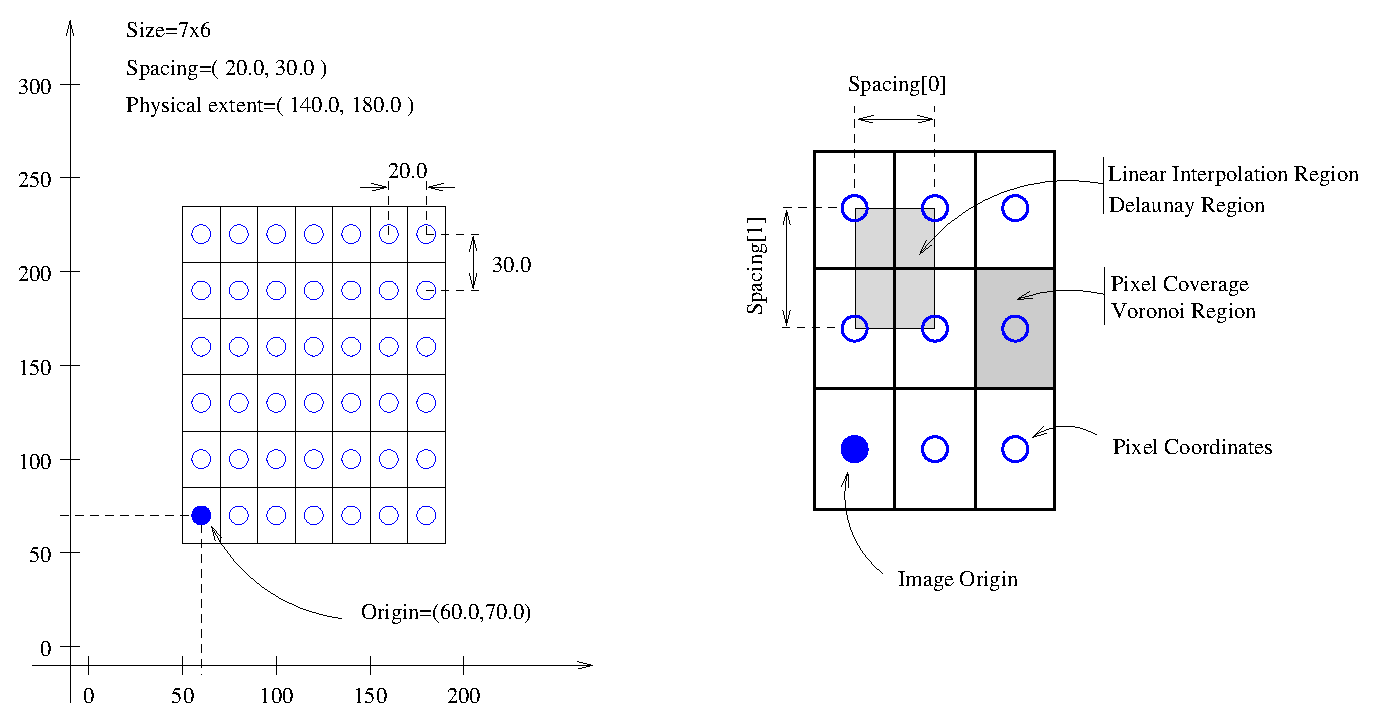
\includegraphics[width=12cm]{images/ImageOriginAndSpacing.eps}
\caption{Geometrical concepts associated with the ITK image.
Adopted from \citet{ITKSoftwareGuideSecondEdition}.}
\label{fig:image}
\end{figure}

Therefore, you should take care that you use an image format that
is able to store the relevant information (e.g. \texttt{mhd},
DICOM). Some image formats, like \texttt{vpx}, do no store the
origin and spacing. This may cause serious problems!

\section{Metrics}\label{sec:comp:metric}

Several choices for the similarity measure can be found in the
literature. Some common choices are described here:

\begin{description}
\item[Sum of Squared Differences (SSD):] The SSD is defined as:
\begin{align}
\mathrm{SSD}(\vmu;I_F,I_M) &= \frac{1}{|I_F|} \sum\limits_{\vx_i
\in I_F} \left( I_F(\vx_i) - I_M(\vT_{\vmu}(\vx_i))
\right)^2,\label{eq:ssd}
\end{align}
with $N$ the number of voxels in the fixed image. Given an
transformation $\vT$, this measure can easily be implemented by
looping over the voxels in the fixed image, taking $I_F(\vx_i)$,
calculating $I_M(\vT_{\vmu}(\vx_i))$ by interpolation, and adding
the squared difference to the sum.

\item[Normalised Correlation Coefficient (NCC):] The NCC is defined as:
\begin{align}
\mathrm{NCC}(\vmu;I_F,I_M) &= \frac{ \sum_{\vx_i \in I_F} \left(
I_F(\vx_i) - \overline{I_F} \right) \left( I_M(\vTm(\vx_i)) -
\overline{I_M} \right) }{ \sqrt{\sum_{\vx_i \in I_F} \left(
I_F(\vx_i) - \overline{I_F} \right)^2 \sum_{\vx_i \in I_F} \left(
I_M(\vTm(\vx_i)) - \overline{I_M} \right)^2} },\label{eq:ncc}
\end{align}
with $\overline{I_F}$ and $\overline{I_M}$ the average grey-value
of $I_F(\vx)$ and $I_M(\vT_{\vmu}(\vx))$, respectively.

\item[Mutual Information (MI):] For MI \citep{MaesEA97,ViolaEA97,MattesEA03} we
use a definition given by \citet{ThevenazEA00a}:
\begin{align}
 MI(\vmu; I_F, I_M) &=
 \sum\limits_{m\in L_M} \sum\limits_{f\in L_F}
 p(f,m;\vmu) \log_2
 \left( \frac{ p(f,m;\vmu) }{ p_F(f) p_M(m;\vmu)  }
 \right),\label{eq:MI}
\end{align}
where $L_F$ and $L_M$ are sets of regularly spaced intensity bin
centres, $p$ is the discrete joint probability, and $p_F$ and
$p_M$ are the marginal discrete probabilities of the fixed and
moving image, obtained by summing $p$ over $m$ and $f$,
respectively. The joint probabilities are estimated using B-spline
Parzen windows:
\begin{align}
\begin{split}
 p(f,m;\vmu) &=  \frac{1}{|I_F|} \sum\limits_{\vx_i \in I_F}
 w_F( f/\sigma_F - I_F(\vx_i)/\sigma_F ) \\
 &\relphantom{=}\times w_M( m/\sigma_M - I_M(\vTm(\vx_i))/\sigma_M ),
\end{split} \label{eq:histogram}
\end{align}
where $w_F$ and $w_M$ represent the fixed and moving B-spline
Parzen windows. The scaling constants $\sigma_F$ and $\sigma_M$
must equal the intensity bin widths defined by $L_F$ and $L_M$.
These follow directly from the grey-value ranges of $I_F$ and
$I_M$ and the user-specified number of histogram bins $|L_F|$ and
$|L_M|$.

\item[Normalized Mutual Information (NMI):] //add description
\cite{Stu99:NMI}

\item[Kappa Statistic (KS):] //add description

\end{description}

The SSD measure is a measure that is only suited for two images
with an equal intensity distribution, i.e. for images from the
same modality. NCC is less strict, it assumes a linear relation
between the intensity values of the fixed and moving image, and
can therefore be used more often. The MI measure is even more
general: only a relation between the probability distributions of
the intensities of the fixed and moving image is assumed. For MI
it is well-known that it is suited not only for mono-modal, but
also for multi-modal image pairs. This measure is often a good
choice for image registration. The NMI measure is, just like MI,
suitable for mono- and multi-modality registration. Literature
\cite{Stu99:NMI} seems to indicate better performance than MI in
some cases. The KS measure is specifically meant to register
binary images (segmentations). It measures the ``overlap'' between
the segmentations.

\section{Sampler}\label{sec:comp:sampler}

In Equations (\ref{eq:ssd})-(\ref{eq:histogram}) we observe a loop
over the fixed image: $\sum_{\vx_i \in I_F}$. Until now, we
assumed that the loop goes over \emph{all} voxels of the fixed
image. In general, this is not necessary. A subset may suffice
\cite{ThevenazEA00a,KleinEA07}. The subset may be selected in
different ways: random, on a grid, etc. The sampler component
represents this process.

The following samplers are often used:
\begin{description}
\item[Full:] A full sampler simply selects all voxel coordinates $\vx_i$ of the
fixed image.

\item[Grid:] The grid sampler defines a regular grid on the fixed
image and selects the coordinates $\vx_i$ on the grid.
Effectively, the grid sampler thus downsamples the fixed image
(not preceded by smoothing, as one would usual do). The dimension
of the grid (or equivalently, the downsampling factor) is a user
input.

\item[Random:] A random sampler randomly selects a user-specified number of
voxels from the fixed image, whose coordinates form $\vx_i$. Every
voxel has equal chance to be selected.

\item[Random Coordinate:] A random coordinate sampler is similar
to a random sampler. It also randomly selects a user-specified
number of coordinates $\vx_i$. However, the random coordinate
sampler is not limited to voxel positions. Also coordinates
between voxels are selected. The grey value $I_F(\vx_i)$ at those
locations must of course be obtained by some interpolation method.

\end{description}

While at first sight the full sampler seems the most obvious
choice, in practice it is not always used, because of its
computational costs in large images. The random samplers are
especially useful in combination with a stochastic optimisation
method \cite{KleinEA07}. See also
Section~\ref{sec:comp:optimiser}. The use of the random coordinate
sampler makes the cost function $\CC$ a more smooth function of
$\vmu$, which makes the optimisation problem (\ref{eq:parametric})
easier to solve. This has been shown in \cite{The08:Halton}.

\section{Transforms}\label{sec:comp:transform}

The transformation model used for $\vT_{\vmu}$ determines what
type of deformations between the fixed and moving image you can
handle. From less flexibility to more we list the translation, the
rigid, the affine, and the nonrigid B-spline transformations.

\begin{description}
\item[Translation:] The translation is defined as:
\begin{align}
\vTmx &= \vx + \bm{t},
\end{align}
with $\bm{t}$ the translation vector. The parameter vector is
simply defined by $\vmu=\bm{t}$.

\item[Rigid:] A rigid transformation is defined as:
\begin{align}
\vTmx &= R \vx + \bm{t},
\end{align}
with the matrix $R$ a rotation matrix, so it is orthonormal and
proper. This means that the image is treated as a rigid body,
which can translate and rotate, but cannot be scaled/stretched.
The rotation matrix is parameterised by the Euler angles (one in
2D, three in 3D). The parameter vector $\vmu$ consists of the
Euler angles and the translation vector. In 2D, this gives a
vector of length 3. In 3D, this gives a vector of length 6.

\item[Similarity:] A similarity transformation is defined as
\begin{align}
\vTmx &= s R \vx + \bm{t},
\end{align}
with $s$ a scalar and $R$ a rotation matrix. This means that the
image is treated as an object, which can translate, rotate, and
scale isotropically. The rotation matrix is parameterised by an
angle in 2D, and by a so-called ``versor'' in 3D (Euler angles
could have been used as well). The parameter vector $\vmu$
consists of the angle/versor, the translation vector, and the
isotropic scaling factor. In 2D, this gives a vector of length 4.
In 3D, this gives a vector of length 7. There are few cases when
you need this transform.

\item[Affine:] An affine transformation is defined as:
\begin{align}
\vTmx &= A \vx + \bm{t},
\end{align}
where the matrix $A$ has no restrictions. This means that the
image can be translated, rotated, scaled, and sheared. The
parameter vector $\vmu$ is formed by the matrix elements $a_{ij}$
and the translation vector. In 2D, this gives a vector of length
6. In 3D, this gives a vector of length 12.

\item[B-splines:] For the category of non-rigid transformations, we focus on a
transformation that is parameterised by B-splines
\citep{RueckertEA99}. In 2D:
\begin{align}
\vTmx = \vx + \sum_{\vx_k \in \NN_{\vx}} \bm{c}_k \bm{\beta}^3(\vx
- \vx_k),\label{eq:bspline}
\end{align}
with $\vx_k$ the control points, $\bm{\beta}^3(x)$ the cubic
multidimensional B-spline polynomial \citep{Unser99}, $\bm{c}_k$
the B-spline coefficient vectors (loosely speaking, the control
point displacements), and $\NN_{\vx}$ the set of all control
points within the compact support of the B-spline at $\vx$. The
control points  $\vx_k$ are defined on a regular grid, overlayed
on the fixed image. In this context we talk about `the control
point grid that is put on the fixed image', and about `control
points that are moved around'. Note that $\vTm(\vx_k)\neq \vx_k +
\bm{c}_k$, a common misunderstanding. Calling $\bm{c}_k$ the
control point displacements is, therefore, actually somewhat
misleading. The control point grid is defined by the amount of
space between the control points, which can be different for each
direction. B-splines have local support ($|\NN_{\vx}|$ is small),
which is beneficial both for modelling local transformations, and
for fast computation. The parameters $\vmu$ are formed by the
B-spline coefficient $\bm{c}_k$. The number of control points
determines the number of parameters. $\approx 10000$ parameters is
not an unusual case.
\end{description}

\begin{figure}
\centering
% was fixed.eps, moving.eps, deformed.eps
\subfigure[fixed]{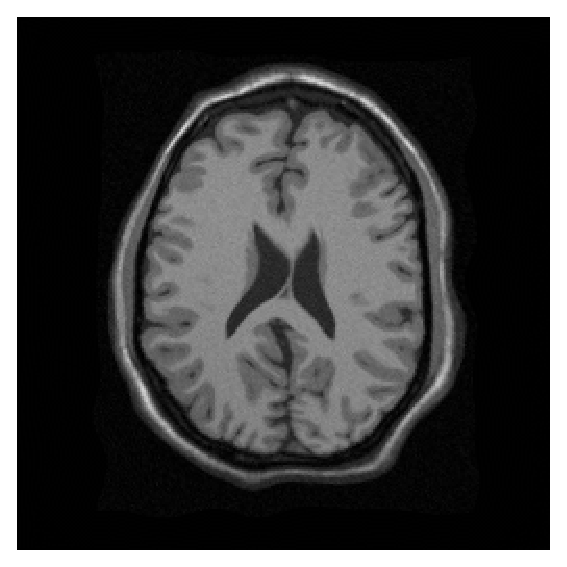
\includegraphics[width=4.5cm,height=4.5cm]{images/transformexample_fixed.eps}}\label{sfig:transformexample:a}
\subfigure[moving]{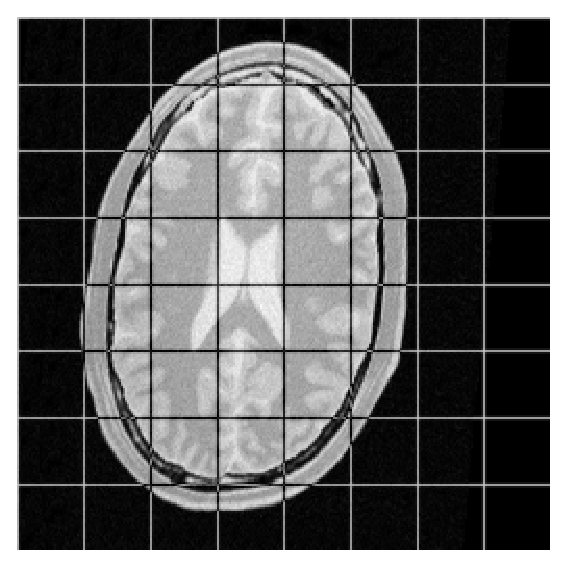
\includegraphics[width=4.5cm,height=4.5cm]{images/transformexample_orig.eps}}\label{sfig:transformexample:b}
\subfigure[translation]{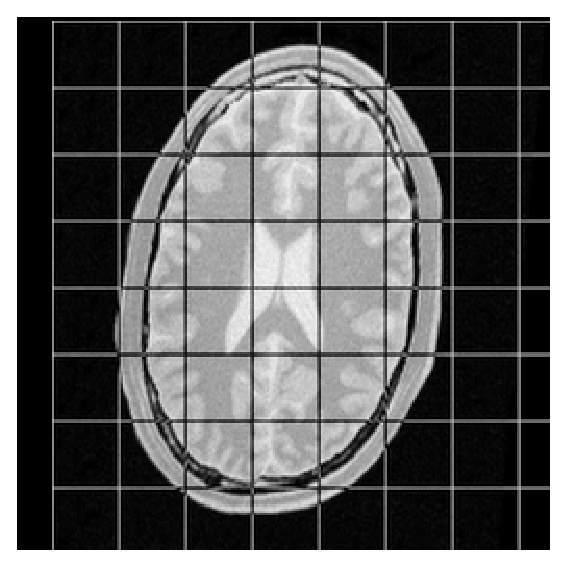
\includegraphics[width=4.5cm,height=4.5cm]{images/transformexample_tran.eps}}\label{sfig:transformexample:c}
\subfigure[rigid]{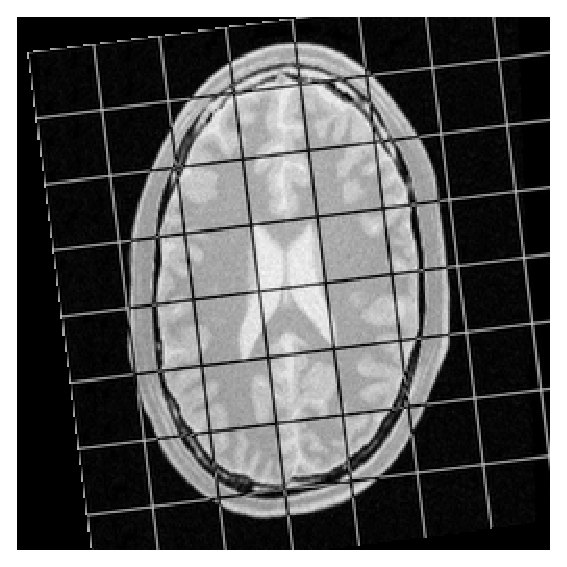
\includegraphics[width=4.5cm,height=4.5cm]{images/transformexample_rig.eps}}\label{sfig:transformexample:d}
\subfigure[affine]{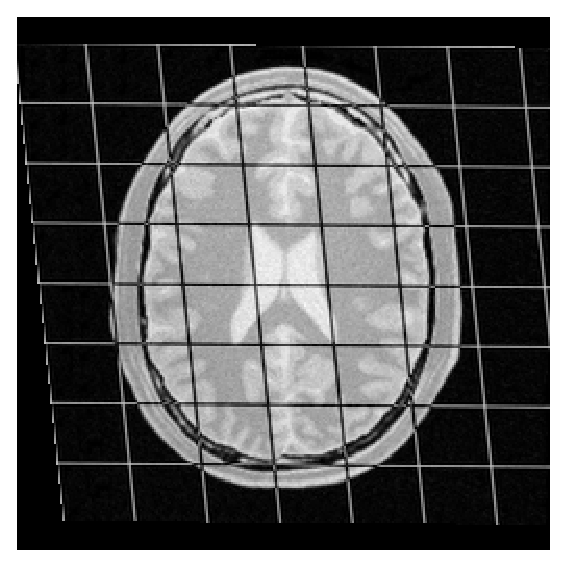
\includegraphics[width=4.5cm,height=4.5cm]{images/transformexample_aff.eps}}\label{sfig:transformexample:e}
\subfigure[B-spline]{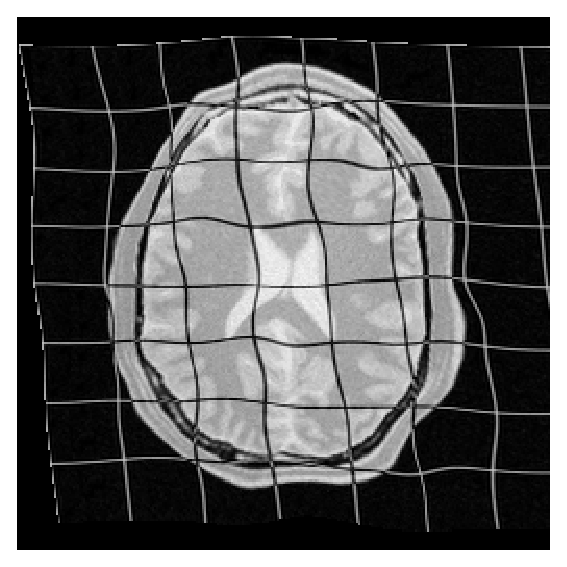
\includegraphics[width=4.5cm,height=4.5cm]{images/transformexample_bsp.eps}}\label{sfig:transformexample:f}
\caption{Different transformations. (a) the fixed image, (b) the
moving image with a grid overlayed, (c) the deformed moving image
$I_M(\vTmx)$ with a translation transformation, (d) a rigid
transformation, (e) an affine transformation, and (f) a B-spline
transformation. The deformed moving image nicely resembles the
fixed image $I_F(\vx)$ using the B-spline transformation. The
overlay grids give an indication of the deformations imposed on
the moving image. NB: the overlayed grid in (f) is NOT the
B-spline control point grid, since that one is defined on the
fixed image!} \label{fig:transformexample}
\end{figure}
See Figure \ref{fig:transformexample} for an illustration of the
different transforms (except for the similarity transformation).
Choose the transformation that fits your needs: only choose a
nonrigid transformation if you expect that the underlying problem
contains local deformations, choose a rigid transformation if you
only need to compensate for differences in pose. To initialise a
nonrigid registration problem, perform a rigid or affine one
first. The result of the initial rigid or affine registration is
combined with the nonrigid B-spline transformation in one of the
following two ways:
\begin{align}
  \text{addition: }\quad    & \vTmx = \vTm^\mathrm{BS}(\vx) + \vT_{\hat\vmu_0}(\vx) \\
  \text{composition: }\quad & \vTmx = \vTm^\mathrm{BS}\left( \vT_{\hat\vmu_0}(\vx) \right)
  = ( \vTm^\mathrm{BS} \circ \vT_{\hat\vmu_0})(\vx)
\end{align}
The latter method is in general to be preferred.

%// iets over scales?


\section{Optimisers}\label{sec:comp:optimiser}

\begin{figure}
\centering
% was: Gradient_descent.eps
\includegraphics[width=0.8\textwidth]{images/gd_example.eps}
\caption{Iterative optimisation. Example for registration with a
translation transformation model. The arrows indicate the steps
$a_k \bm{d}_k$ taken in the direction of the optimum, which is the
minimum of the cost function.} \label{fig:optimisation}
\end{figure}
To solve the optimisation problem (\ref{eq:parametric}), i.e. to
obtain the optimal transformation parameter vector $\hat\vmu$,
commonly an iterative optimisation strategy is employed:
\begin{align}
\vmu_{k+1} &= \vmu_k + a_k \bm{d}_k, \quad k = 0, 1, 2, \cdots,
\end{align}
with $\bm{d}_k$ the `search direction' at iteration $k$, $a_k$ a
scalar gain factor controlling the step size along the search
direction. The optimisation process is illustrated in Figure
\ref{fig:optimisation}. \citet{KleinEA07} give an overview of
various optimisation routines the literature offers. Examples are
quasi-Newton (QN), nonlinear conjugate gradient (NCG), gradient
descent (GD), and Robbins-Monro (RM). Gradient descent and
Robbins-Monro are discussed below. For details on other
optimisation methods we refer to \citep{KleinEA07,NocedalEA99}.

\begin{description}
\item[Gradient descent (GD):] Gradient descent optimisation methods take the
search direction as the negative gradient of the cost function:
\begin{align}
\vmu_{k+1} &= \vmu_k - a_k \bm{g}(\vmu_k),\label{eq:gd}
\end{align}
with $\bm{g}(\vmu_k) = \partial \mathcal{C} / \partial \vmu$
evaluated at the current position $\vmu_k$. Several choices exist
for the gain factor $a_k$, such as a determined by a line search
or using a predefined function of $k$.

\item[Robbins-Monro (RM):] The RM optimisation method replace the calculation of
the derivative of the cost function $\bm{g}(\vmu_k)$ by an
approximation $\widetilde{\bm{g}}_k$.
\begin{align}
\vmu_{k+1} &= \vmu_k - a_k \widetilde{\bm{g}}_k,\label{eq:RM}
\end{align}
The approximation is potentially faster to compute, but might
deteriorate convergence properties of the GD scheme.
\citet{KleinEA07} showed that using only a small random subset of
voxels ($\approx 2000$) from the fixed image accelerates
registration significantly, without compromising registration
accuracy. The Random or RandomCoordinate samplers, described in
Section~\ref{sec:comp:sampler}, are examples of samplers that pick
voxels randomly. It is important that a new subset of fixed image
voxels is selected every iteration $k$, so that the approximation
error has zero mean. The RM method is usually combined with $a_k$
as a predefined decaying function of $k$:
\begin{align}
a_k &= \frac{a}{(k+A)^{\alpha}},\label{eq:gain}
\end{align}
where $a > 0$, $A \ge 1$, and $0 \le \alpha \le 1$ are
user-defined constants. In our experience, a reasonable choice is
$\alpha = 0.602$ and $A$ approximately 10\% of the user-defined
maximum number of iterations, or less. The choice of the overall
gain, $a$, depends on the expected ranges of $\vmu$ and $\bm{g}$
and is thus problem specific.
\end{description}

Note that GD and RM are in fact very similar. Running RM with a
Full sampler (see Section~\ref{sec:comp:sampler}), instead of a
Random sampler, is equivalent to performing GD. We recommend the
use of RM over GD, since it is so much faster, without
compromising on accuracy. In that case, the parameter $a$ is
parameter that is to be tuned for your application.

\section{Interpolators}\label{sec:comp:interpolator}

As stated above, during the optimisation the value $I_M(\vTmx)$ is
evaluated at non-voxel positions, for which intensity
interpolation is needed. Several methods for interpolation exist,
varying in quality and speed. Some examples are given in Figure
\ref{fig:interpolation}.

\begin{description}
\item[Nearest neighbour:] This is the most simple technique, low in
quality, requiring little resources. The intensity of the nearest
voxel is returned.

\item[Linear:] Still very simple. The returned value is a weighted
average of the surrounding voxels, with the distance to each voxel
taken as weight.

\item[$N$-th order B-spline:] The higher the order, the better the
quality, but also requiring more computation time. See
\citet{Unser99} for more details.
\end{description}

During registration a first order B-spline interpolation, i.e. linear
interpolation, often gives satisfactory results. It is a good
trade-off between quality and speed. To generate the final result,
i.e. the deformed result of the registration, a higher order
interpolation is usually required, for which we recommend $N=3$.

\begin{figure}
\centering
\subfigure[]{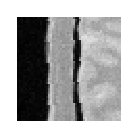
\includegraphics[width=2.5cm]{images/nn.eps}}\label{sfig:interpolation:nn}
\subfigure[]{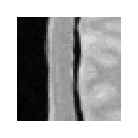
\includegraphics[width=2.5cm]{images/linear.eps}}\label{sfig:interpolation:lin}
\subfigure[]{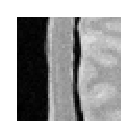
\includegraphics[width=2.5cm]{images/bs2.eps}}\label{sfig:interpolation:bs2}
\subfigure[]{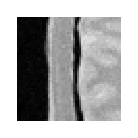
\includegraphics[width=2.5cm]{images/bs3.eps}}\label{sfig:interpolation:bs3}
\subfigure[]{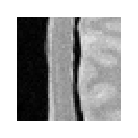
\includegraphics[width=2.5cm]{images/bs5.eps}}\label{sfig:interpolation:bs5}
\caption{Interpolation. (a) nearest neighbour, (b) linear, (c) B-spline $N=2$,
(d) B-spline $N=3$, (e) B-spline $N=5$.} \label{fig:interpolation}
\end{figure}

\section{Multi-resolution}\label{sec:comp:multiresolution}

For a good overview of multi-resolution strategies see
\citet{LesterEA99}. Two hierarchical methods are distinguished:
reduction of data complexity, and reduction of transformation
complexity.

\subsection{Data complexity}

It is common to start the registration process using images that
have lower complexity, e.g., images that are smoothed and possibly
downsampled. This increases the chance of successful registration.
A series of images with increasing amount of smoothing is called a
scale space. If the images are not only smoothed, but also
downsampled the data is not only less complex, but the
\emph{amount} of data is actually reduced. In that case, we talk
about an ``pyramid''. However, confusingly, the word pyramid is
used by us also to refer to a scale space. Several scale spaces or
pyramids are found in the literature, amongst others Gaussian and
Laplacian pyramids, morphological scale space, and spline and
wavelet pyramids. The Gaussian pyramid is the most common one.
Figure~\ref{fig:multiresolution} shows the Gaussian pyramid with
and without downsampling. In combination with a Full sampler (see
Section~\ref{sec:comp:sampler}), using a pyramid with downsampling
will save a lot of times in the first resolution levels, because
the image contains much less voxels. In combination with a Random
sampler, or RandomCoordinate, the downsampling step is not
necessary, since the random samplers anyway select a user-defined
number of samples, independent of the image size.
\begin{figure}
\centering
\subfigure[resolution 0]{
\includegraphics[width=3cm]{images/moving_pd.R0d.eps}}
\subfigure[resolution 1]{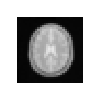
\includegraphics[width=3cm]{images/moving_pd.R1d.eps}}
\subfigure[resolution 2]{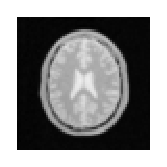
\includegraphics[width=3cm]{images/moving_pd.R2d.eps}}
\subfigure[original]{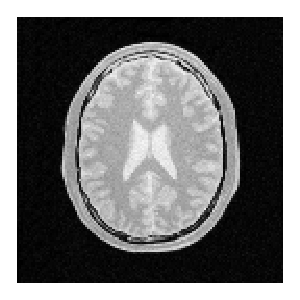
\includegraphics[width=3cm]{images/moving_pd.128.eps}} \\
\subfigure[resolution 0]{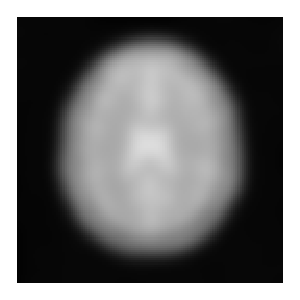
\includegraphics[width=3cm]{images/moving_pd.R0.eps}}
\subfigure[resolution 1]{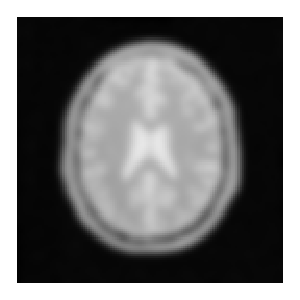
\includegraphics[width=3cm]{images/moving_pd.R1.eps}}
\subfigure[resolution 2]{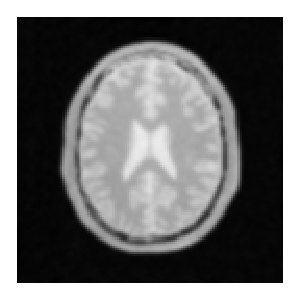
\includegraphics[width=3cm]{images/moving_pd.R2.eps}}
\subfigure[original]{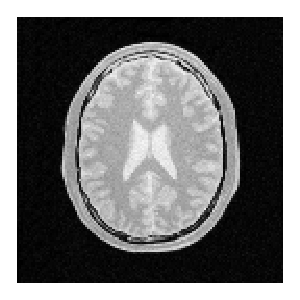
\includegraphics[width=3cm]{images/moving_pd.128.eps}}
\caption{Two multi-resolution strategies using a Gaussian pyramid ($\sigma = 8.0, 4.0, 2.0$
voxels). The first row shows multi-resolution with down-sampling, the
second row without. Note that for the first row the image size is
halved every resolution, but that the voxel size increases with a
factor 2, so physically the images are of the same size every
resolution.} \label{fig:multiresolution}
\end{figure}


\subsection{Transformation complexity}

The second multiresolution strategy is to start the registration
with fewer degrees of freedom for the transformation model. The
degrees of freedom of the transformation equals the length (number
of elements) of the parameter vector $\vmu$.

An example of this was already mentioned in
Section~\ref{sec:comp:transform}: the use of a rigid
transformation prior to nonrigid B-spline registration. We may
even use a three-level strategy: first rigid, then affine, then
nonrigid B-spline.

Another example is to increase the number of degrees of freedom
within the transformation model. With a B-spline transformation,
it is often good practice to start registration with a coarse
control point grid, only capable of modelling coarse deformations.
In subsequent resolutions the B-spline grid is gradually refined,
thereby introducing the capability to match smaller structures.

%%%%%%%%%%%%%%%%%%%%%%%%%%%%%%%%%%%%%%%%%%%%%%%%%%%%%%%%%%%%%%%%%%%%%%%%%%%%%%%%%%%%%%%%%%%%

\chapter{\elastix}\label{chp:elastix}

\section{Introduction}

The development of \elastix\ started half to late 2003, and was
intended to facilitate our registration research. After some initial
versions we decided to put the separate components of \elastix\ in
separate libraries. This resulted in major version 3.0 in November
2004. \elastix\ 3.0 was also the first version that was made publicly
available on the \elastix\ website, around the same time. The
continued development brings us today (December 2007) to version 3.8.

\begin{tabular}{l|l}
what & where \\
\hline
website        & \url{www.isi.uu.nl/Elastix} \\
CVS repository & \url{/shared/CVS/elastix/} (hosted at the ISI) \\
WIKI           & \url{https://wiki.isi.uu.nl/bin/view/CADweb/ElastiX} \\
FAQ            &
\url{https://wiki.isi.uu.nl/bin/view/CADweb/ElastixFAQ}
\end{tabular}

The website also contains a doxygen\footnote{\url{www.doxygen.org}}
generated part that provides documentation of the source code. An
overview of all available classes can be found at
\begin{quote}
\url{www.isi.uu.nl/Elastix/doxygen/classes.html}.
\end{quote}
For each class a description of this class is given, together with
information on how to use it in \elastix. See
\begin{quote}
\url{www.isi.uu.nl/Elastix/doxygen/modules.html}
\end{quote}
for an overview of all available components.

\subsection{Key features}

\elastix\ is
\begin{itemize}
\item open source, freely available from \url{www.isi.uu.nl/Elastix};

\item based on the ITK, so the code base is thoroughly tested, nightly.
But with some improvements.

\item multi-platform (at least Windows, Linux, Mac OS ??), multi-compiler
(at least Visual C++ 2003, gcc 3.2, gcc 4.02), and supports 32 and 64
bit systems. So, it is highly portable to the platform of the users
choice;

\item highly configurable, which is easy thanks to human
readable/edible parameter file;

\item easy to use for large amounts of data, since \elastix\ can be
called easily in a script;

\item fast, thanks to subsampling, if desired;

\item relatively easy to extend, i.e. to add new components, so it is
very suited for research also.
\end{itemize}

\section{How to call \elastix}

\elastix\ is a command line program. This means that you have to open
a command line interface (a DOS-box, a shell) and type in an
appropriate elastix command. This also means that there is no
graphical user interface. Help on using the program can be acquired
as follows:
\begin{quote}
\texttt{elastix --help}
\end{quote}
which will give a list of mandatory and optional arguments. The most
basic command to run a registration is as follows:
\begin{quote}
\texttt{elastix -f fixedImage.ext -m movingImage.ext -out
outputDirectory -p parameterFile.txt}
\end{quote}
where `\texttt{ext}' is the extension of the image files. The above
arguments are mandatory. These are minimally needed to run \elastix.
All output of \elastix\ is written to the output directory, which
needs to be created before running \elastix. The output consists of a
log file (\texttt{elastix.log}), and optionally the resulting
registered image (\texttt{result.?.mhd}), the parameters of the
transformation that relate the fixed and the moving image
(\texttt{TransformParameters.?.txt}). The parameter file is an
important file: in it is defined, in normal text, what kind of
registration is performed (i.e. what metric, optimizer, etc.) and
what the parameters are that define the registration. It gives a high
amount of flexibility and control over the process. More information
about the parameter file is given in Section \ref{sec:elastix:param}.

The use of masks is supported. They can be provided by adding
\texttt{-fMask fixedMask.ext} and/or \texttt{-mMask movingMask.ext}
to the command line. An initial transformation can be provided with a
valid transform parameter file by adding \texttt{-t0
TransformParameters.txt} to the command line. With the command line
option \texttt{-threads unsigned\_int} the user can specify the
maximum number of threads that \elastix\ will use.

On the \elastix\-website, in the `About' section, you can find an
example on how to use the program. Maybe now is the time to try the
example and see a registration in action.

Running multiple registrations in succession, each possibly of a
different type, and with the output of a previous registration as
input to the next, can be done with \elastix\ in several ways. The
first one is to run \elastix\ once with the first registration, and
use its output (the \texttt{TransformParameter.0.txt} that can be
found in the output directory) as input for a new run of \elastix\
with the command line argument \texttt{-t0}. So:
\begin{quote}
\texttt{elastix -f ... -m ... -out out1 -p param1.txt} \\
\texttt{elastix -f ... -m ... -out out2 -p param2.txt -t0
out1/TransformParameters.0.txt} \\
\texttt{elastix -f ... -m ... -out out3 -p param3.txt -t0
out2/TransformParameters.0.txt}
\end{quote}
and so on. Another possibility is combine the registrations with one
run of \elastix:
\begin{quote}
\texttt{elastix ... -p param1.txt -p param2.txt -p param3.txt}
\end{quote}
The transformations from each of the registrations are automatically
combined.

\section{General code layout}

\section{The parameter file}\label{sec:elastix:param}

The parameter file is a text file that defines the components of the
registration and their parameter values. Supplying a parameter works
as follows:
\begin{quote}
\texttt{(ParameterName value(s))}
\end{quote}
So parameters are provided between brackets, first the name, followed
by one or more values. If the value if of type string then the values
need to be quoted: \texttt{(ParameterName "value1" ... "valueN")}. If
the values are of floating type, then at least one value behind the
comma need to be given: \texttt{(ParameterName 1.3 3.0)}. Comments
can be provided by adding `\texttt{//}' before a line. A minimal
example of a valid parameter file is given in Appendix \ref{chp:ExampleParam}.
A list of available parameters for each class is given at
\texttt{www.isi.uu.nl/Elastix/doxygen/parameter.html}.

Since the choice of the several components and the parameter values
define the registration, it is very important to set them wisely.
These choices is what makes the registration a success or a disaster.
Therefore, a separate chapter is dedicated to the fine art of tuning
a registration, see Chapter \ref{chp:Tutorial}.

%%%%%%%%%%%%%%%%%%%%%%%%%%%%%%%%%%%%%%%%%%%%%%%%%%%%%%%%%%%%%%%%%%%%%%%%%%%%%%%%%%%%%%%%%%%%

\chapter{\transformix}\label{chp:transformix}

\section{Introduction}

By now you are able to at least run a registration, by calling
\elastix\ correctly. It is often also useful to apply the
transformation as found by the registration to another image. Maybe
you want to apply the transformation to an original larger image to
gain resolution. Or maybe you need the transformation to apply it to
an atlas image. For those purposes a program called \transformix\ is
available. It was developed simultaneously with \elastix.

\section{How to call \transformix}

Like \elastix\, \transformix is a command line driven program. You
can get basic help on how to call it, by:
\begin{quote}
\texttt{transformix --help}
\end{quote}
which will give a list of mandatory and optional arguments. The most
basic command is as follows:
\begin{quote}
\texttt{transformix -in inputImage.ext -out outputDirectory -tp
TransformParameters.txt}
\end{quote}
This call will transform the input image and write it, together with
a log file, to the output directory. The transformation you want to
apply is defined in the so-called transform parameter file, see
Section \ref{sec:transformix:tp}. If you want to deform a set or all
points, the appropriate call is:
\begin{quote}
\texttt{transformix -ipp inputPoints.txt -out outputDirectory -tp
TransformParameters.txt} \\
\texttt{transformix -ipp all -out outputDirectory -tp
TransformParameters.txt}
\end{quote}
This will create a file the deformed output points or a deformation
field vector image. With the command line option \texttt{-threads
unsigned\_int} the user can specify the maximum number of threads
that \transformix\ will use.

\section{Details}

The run-time of \transformix\ is built up of the following parts:

1. computing the B-spline decomposition 2. computing the deformation
for each voxel 3. interpolating the input image for each voxel.

I'm not sure, but I guess step 2 is the most time-consuming task, in
case of a B-spline deformation. For a nD B-spline deformation,
computing the deformation vector at a voxel basically amounts to n
interpolations.

Step 1. is avoided by using a linear interpolator of course.

Step 3 is faster when using linear interpolation instead of cubic
interpolation. I don't know how much exactly.

What is the complexity of FinalBSplineInterpolator? And of
FinalLinearInterpolator? In required operations per voxel. Is that
described in the docs, in some papers, or on the wiki?

Memory consumption, see the wiki

\section{The transform parameter file}\label{sec:transformix:tp}

The result of a registration is the transformation relating the fixed
and moving image. The parameters of this transformation are stored in
a \texttt{TransformParameters.?.txt}-file. An example of its
structure for a 2D rigid transformation is given in Appendix
\ref{chp:ExampleTransformParam}. The text file contains all
information necessary to resample an input image (the moving image)
to the region specified in the file (by default the fixed image
region).

The transform parameter file can be manually edited or created as is
convenient for the user. Multiple transformations are composed by
iteratively supplying another transform parameter file with the
\texttt{InitialTransformParametersFileName} tag.

%%%%%%%%%%%%%%%%%%%%%%%%%%%%%%%%%%%%%%%%%%%%%%%%%%%%%%%%%%%%%%%%%%%%%%%%%%%%%%%%%%%%%%%%%%%%

\chapter{Tutorial}\label{chp:Tutorial}


\section{General advice}

When performing registration one carefully has to choose the several
components, as specified in Chapter \ref{chp:Registration}. In Table
\ref{table:tutorial:components} some recommendations are given.

\begin{table}[htb]
\centering
\begin{tabular*}{15cm}{@{\extracolsep{\fill}} p{3.5cm} | p{11cm} }
\textbf{Component} & \textbf{Recommendation} \\
\hline
Registration & \texttt{MultiResolutionRegistration}: Multiple image
resolutions is what you need, 3 or more is a good starting point. And
if you think you don't need all this multi-resolution, you can always
set the \texttt{NumberOfResolutions} to 1. \\
FixedImagePyramid & \texttt{FixedSmoothingImagePyramid}: this pyramid
will smooth, but not down-sample the fixed image for you, according
to the \texttt{FixedImageSchedule} you provide. If you only set the
\texttt{NumberOfResolutions}, a default schedule will be used that
down-samples the fixed image by 2. That schedule is usually fine. In
case you have highly anisotropic data, you might want to blur less in
the direction of the largest spacing. \\
MovingImagePyramid & See the FixedImagePyramid. \\
Metric    & \texttt{AdvancedMattesMutualInformation}: usually works
well, both for mono- and multi-modal images. It supports fast
computation of the metric value and derivative in case the transform
is a B-spline. \\
Optimizer & \texttt{StandardGradientDescent}: see Equations
(\ref{eq:gd}) and (\ref{eq:gain}). Offers the possibility to perform
fast registration, see \cite{KleinEA07}. The problem is to tune the
parameters of the gain factor $a_k$, see Section
\ref{sec:Tutorial:importantparam}. \\
Sampler & \texttt{RandomCoordinate}: works well in conjunction with
the \texttt{StandardGradientDescent} optimiser. Set the
\texttt{NumberOfSpatialSamples} to 3000. \\
Transform & Depends on the application. For rigid choose
\texttt{EulerTransform}, for affine \texttt{AffineTransform}, for
nonrigid registration problems \elastix\ has the
\texttt{BSplineTransform}. The latter requires setting the
\texttt{FinalGridSpacing}. Always start with a rigid or affine
transformation before doing a nonrigid one, to get a good initial
alignment. \\
Interpolator & \texttt{BSplineInterpolator}: first order is usually
enough during the registration: \texttt{(BSplineInterpolationOrder
1)}. \\
ResampleInterpolator & \texttt{FinalBSplineInterpolator}: the
interpolator that is used for generating the resulting deformed
moving image. We recommend a third order B-spline for this:
\texttt{(FinalBSplineInterpolationOrder 3)}.
\end{tabular*}
\caption{Some recommendations for the several components.}\label{table:tutorial:components}
\end{table}

\section{Overview of all parameters}

A list of all parameters that can be specified for each registration
component can be found at the \elastix\ website:
\begin{quote}
\url{www.isi.uu.nl/Elastix/doxygen/parameter.html}
\end{quote}
At that site you can find how to specify a parameter and what the
default value is. We have tried to come up with sensible defaults,
although the defaults will not work in all cases.


\section{Important parameters}\label{sec:Tutorial:importantparam}

\begin{description}
\item[On multi-resolution:] Two parameters have to be set to define
the multi-resolution strategy: the number of resolutions and the
specific down-sampling schedule that is used in each resolution.

In general 3 resolutions is a good starting point. If the fixed and
moving image are initially far away, you can increase the number of
resolution levels to, say, 5 or 6. This way the images are more
blurred and more attention is paid to register large, dominant
structures.

The pyramid schedule defines the amount of blurring, and
down-sampling in case of a FixedRecursiveImagePyramid is used, in
each direction $x,y,z$ and for each resolution level. It can be
specified as follows:
\begin{quote}
\texttt{(FixedImagePyramidSchedule 8 8 4 4 2 2 1 1)}
\end{quote}
In this example 4 resolutions for a 2D image are used. At resolution
level 0 the image is, possibly, downsampled by a factor 8 and blurred
with $\sigma = 8/2$ voxels in each direction. At level 1 a factor 4
is used, and finally at the last level, level 4, the original images
are used for registration. Specifying the fixed and moving image
pyramids with an identical schedule can be done with one command,
e.g.:
\begin{quote}
\texttt{(ImagePyramidSchedule 4 4 2 2 2 1 1 1 1)}
\end{quote}
for a 3D image with 3 resolution levels, where less smoothing is
performed in the $z$-direction.

\item[On multi-grid:] The B-spline nonrigid transformation is defined
by a uniform grid of control points. This grid is defined by the
spacing between the grid nodes. The spacing defines how dense the
grid is, or what the locality is of the transformation you can model.
For each resolution level you can define a different grid spacing.
This is what we call multi-grid. In general, we recommend to start
with a coarse B-spline grid, i.e. a more global transformation. This
way first the larger structures are matched, for the same reason as
why you should start with a rigid or affine transformation. In later
resolutions you can refine the transformation in a stepwise fashion;
the idea is that you subsequently match smaller structures, up to the
final precision. The final grid spacing is specified with:
\begin{quote}
\texttt{(FinalGridSpacingInPhysicalUnits 10.0 10.0 10.0)}
\end{quote}
with as much numbers as there are dimensions in your image. The
spacing is in most medical images specified in millimetres. It is
also possible to specify the grid in voxel units:
\begin{quote}
\texttt{(FinalGridSpacingInVoxels 16.0 16.0 16.0)}
\end{quote}
If the final B-spline grid spacing is chosen high, then you cannot
match small structures. On the other hand, if the grid spacing is
chosen very low, then small structures can be matched, but you
possibly allow the transformation too have too much freedom. This can
result in irregular transformations, especially on homogenous parts
of your image, since there are no edges (or other information) at
such areas that can guide the registration. A penalty or
regularisation term, see Equation (\ref{eq:registration2}), can help
to avoid these problems. It is hard to recommend a value for the
final grid spacing, since it depends on the desired accuracy. But we
can try: if you are interested in somewhat larger structures, you
could set it too 32 voxels, for matching smaller structures you could
go down to 16 or 8 voxels, or even up to 4. The last choice will
maybe require some regularisation term, unless maybe if you have
carefully and gradually refined the grid spacing.

To specify a multi-grid schedule use the \texttt{GridSpacingSchedule}
command:
\begin{quote}
\texttt{(NumberOfResolutions 4)} \\
\texttt{(FinalGridSpacingInVoxels 8.0 8.0)} \\
\texttt{(GridSpacingSchedule 6.0 6.0 4.0 4.0 2.5 2.5 1.0 1.0)}
\end{quote}
In case of 2D images, this schedule specifies a grid spacing of $6
\times 8 = 48$ voxels in resolution level 0, via 32 and 20 voxels, to
8 voxels in the final resolution level.

As a side-note: the number of parameters that are minimised in
(\ref{eq:registration1}) is determined by the size of $\vmu$, i.e. in
case of the B-spline deformable transform by the control point grid
spacing. If you double the spacing, the number of parameters are
increased by a factor 8 for a 3D image. For a $256^3$ image and a
grid spacing of 16 voxels this will result in approximately
$(256/16)^3 \times 3 \approx 12.000$ parameters; for a grid spacing
of 8 voxels this is almost 100.000 parameters. The amount of
parameters is directly related to memory consumption and registration
time.

\item[On the sampler:] The recommended optimisation routine is the
\texttt{StandardGradientDescent} method. This method can be used with
a small amount of samples, randomly selected in every iteration, see
Section ???, which significantly decreases registration time. We
recommend:
\begin{quote}
\texttt{(ImageSampler "RandomCoordinate")} \\
\texttt{(NumberOfSpatialSamples 3000)}
\end{quote}
The first line selects a sampler that draws samples from the fixed
image. These samples are not necessarily on voxel locations (on the
voxel grid), but are mostly from points between voxels, so
interpolation is needed. This specific sampler avoids what is known
as the grid-effect [citations]. The second line specifies that 3000
samples are drawn, which is enough to get a convergence as fast as
using all samples, but of course with a significantly reduced
computation time per iteration.

\item[On the optimiser:] The \texttt{StandardGradientDescent} method
(\ref{eq:RM}) needs a choice for the step size $a_k$, which is in
\elastix\ defined as in Equation (\ref{eq:gain}). For the parameter
$\alpha$ we recommend the value 0.602. For $A$, use something in the
order of 50. This leaves the parameter $a$ as the most important
parameter to tune. And it is an important parameter, it can mean
success for a good choice and failure if not! If $a$ is set too high,
the iterative solving algorithm (\ref{eq:RM}) becomes unstable, and
you may deform your image beyond recognition. If $a$ is set too low,
you will never make it to the optimum, or may get stuck in a very
small nearby local optimum. Too complicate things further, a good
choice for $a$ is dependent on the cost function that is used for
registration: the $a$ that will give you a good result for SSD is not
the same as the one that gives a good result for MI. Finally, $a$
also depends on the amount of deformation that you expect between the
fixed and the moving image. So again, recommendations are hard to
give. In general we advise you to think in orders of magnitude, if $a
= 10$ is too small, try $a = 100$ and not $a = 11$. For mutual
information you could start around $a = 1000.0$. For the mean squared
difference metric you could try something smaller than 1 ???
\begin{quote}
\texttt{(SP\_a 1000.0 500.0 500.0)} \\
\texttt{(SP\_alpha 0.602)} \\
\texttt{(SP\_A 50.0)}
\end{quote}
$a$ equally large for every resolution level? or start with large
steps end with small steps?

number of iterations
\begin{quote}
\texttt{(MaximumNumberOfIterations 500)}
\end{quote}
which is not only the maximum, but also the minimum, since there is
no other appropriate stopping condition for this optimiser.

\end{description}


\section{Masks}

when to use masks

when not to use masks

when to use erosion during multi-resolution and when not

Common errors when drawing samples from the fixed image with small
mask.


\section{Trouble shooting}

\subsection{Bad initial alignment}

\begin{figure}
\centering \psfrag{k}[tc][tc]{$k$} \psfrag{ak}[tc][tc]{$a_k$}
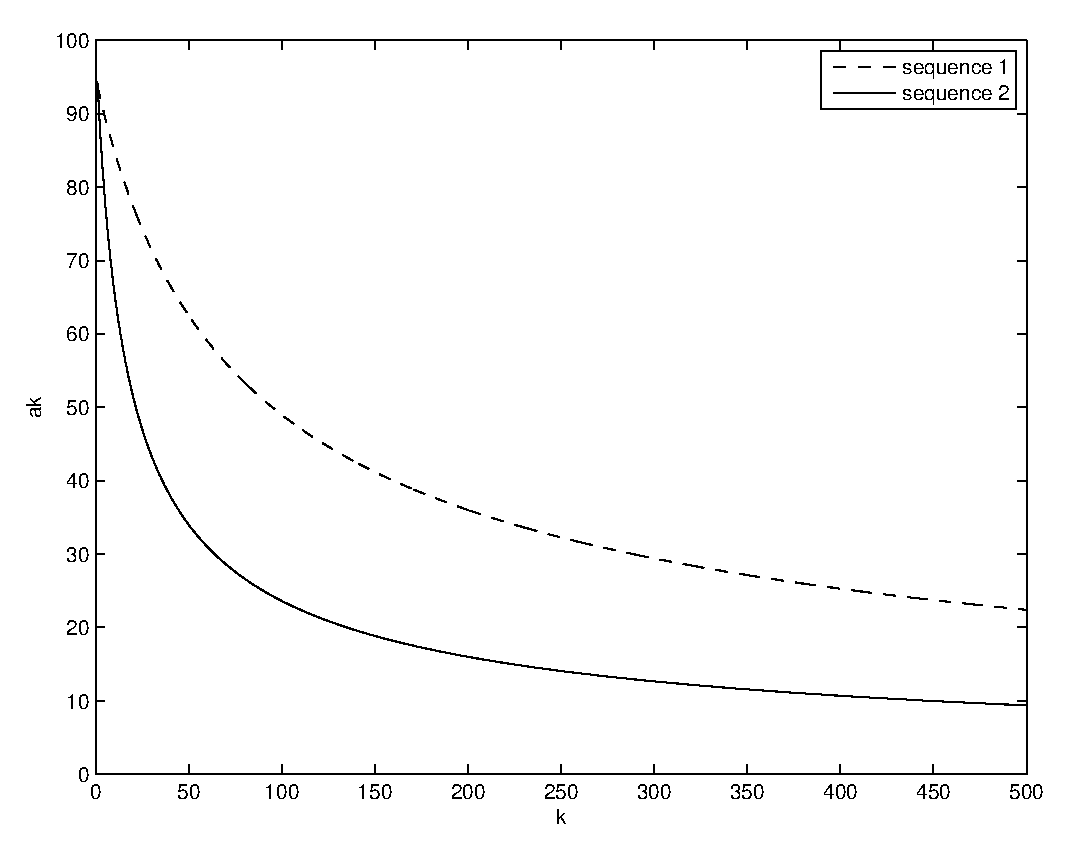
\includegraphics[width=8cm]{images/ak.eps}
\caption{Sequence 1: $a = 1000$, $A = 50$, $\alpha = 0.602$.
Sequence 2: $a = 400$, $A = 10$, $\alpha = 0.602$. Both sequences
start with the same step size, but sequence 2 decays much
faster.}\label{fig:ak}
\end{figure}

When the initial alignment between two images is very off, you cannot
start a nonrigid registration. And sometimes it can be a hassle to
get it right. What factors can help to get it right?

\begin{itemize}
\item So you choose a transformation with a low degree of freedom,
i.e. the translation, rigid, similarity or affine transform.

\item You need a good multi-resolution strategy, i.e.
quite a bit of resolution levels. This way a lot of smoothing is
going on, blurring away all the details and thereby focussing the
registration on the major structures.

\item You can afford to take large steps now, so do it. Set the
parameter $a$ so high that the translation component of the
transformation takes a step of several voxels in each iteration, up
to 10. Maybe it will work, and in that case you will get alignment
pretty quick, but the step size $a$ is still large, so you
immediately jump away from alignment again. If that happens, you
should let the sequence $a_k = a / (A+k)^{\alpha}$ decay relatively
fast. This can be achieved by setting both $a$ and $A$ a bit lower,
see Figure \ref{fig:ak}.

\item In case you need to find a large rotation, you might want to
take larger steps for the rotation, but not for the translation. This
can be achieved by modifying the scales parameter, see Section ???:
\begin{quote}
\texttt{(Scales 10000.0)}
\end{quote}
You can set it lower to take larger rotation steps. If it is set to
1.0 you take as large steps for the rotation as for the translation
(but the rotation is defined in radials). If you set it really high
($> 10^6$) you won't rotate at all. You probably don't need to go
lower than 1000.0.

\end{itemize}

\subsection{Memory consumption}

The typical size of clinical images increases as a function of time.
Therefore, memory efficiency will become more of an issue. \elastix\
consumes $\approx$ 100 MB of memory for small images, for larger
image pairs ($256^3$) and some common components, consumption can be
about 1 - 1.5 GB. With very large images ($400^3$ and above) memory
consumption can rise above the 2 GB limit of most Windows systems.
What to do with large images?
\begin{itemize}
\item Buy yourself a brand new computer with a lot of memory. Make
sure that this computer is 64 bit, otherwise you cannot address this
much memory. Also make sure that your operating system supports 64
bit.

\item Images in \elastix\ are internally by default represented as a bunch of
voxels of floating type. You can modify this to short images:
\begin{quote}
\texttt{(FixedInternalImagePixelType "short")} \\
\texttt{(MovingInternalImagePixelType "short")}
\end{quote}
This way you save half the amount of memory that is used to store the
fixed and moving images, and their multi-resolution pyramids. This
will come at the cost of a loss of precision, but may not be that
harmful. This option is useful both for \elastix\ and \transformix.

\item Change the interpolator that is used during registration. By default a B-spline
interpolator is used, which stores a coefficient image internally in
double type. You can also specify a float version:
\begin{quote}
\texttt{(Interpolator "BSplineInterpolatorFloat")}
\end{quote}
which saves you another bit of memory the size of a short image. This
option is useful for \elastix\ only.

\item Change the interpolator that is used when resampling an image:
\begin{quote}
\texttt{(ResampleInterpolator "FinalBSplineInterpolatorFloat")}
\end{quote}
This option is useful both for \elastix\ and \transformix. However,
for \elastix\ it will only save you some memory at the very end of
the registration.

\end{itemize}


\subsection{Common errors}

Some common sources of confusion and questions have been gathered in
a FAQ, which can be found at
\begin{quote}
\url{www.isi.uu.nl/Elastix/FAQ.php}
\end{quote}


\section{Example}

Step-by-step example where we give a look into our head, what magical
thoughts we think when tuning the registration.


%%%%%%%%%%%%%%%%%%%%%%%%%%%%%%%%%%%%%%%%%%%%%%%%%%%%%%%%%%%%%%%%%%%%%%%%%%%%%%%%%%%%%%%%%%%%

\chapter{Developers guide}\label{chp:develop}

\section{Setup of the code}

\section{Creating new modules}

%%%%%%%%%%%%%%%%%%%%%%%%%%%%%%%%%%%%%%%%%%%%%%%%%%%%%%%%%%%%%%%%%%%%%%%%%%%%%%%%%%%%%%%%%%%%

\appendix

\chapter{Example parameter file}\label{chp:ExampleParam}

\begin{verbatim}
//ImageTypes
(FixedInternalImagePixelType "float")
(FixedImageDimension 2)
(MovingInternalImagePixelType "float")
(MovingImageDimension 2)

//Components
(Registration "MultiResolutionRegistration")
(FixedImagePyramid "FixedRecursiveImagePyramid")
(MovingImagePyramid "MovingRecursiveImagePyramid")
(Interpolator "BSplineInterpolator")
(Metric "AdvancedMattesMutualInformation")
(Optimizer "StandardGradientDescent")
(ResampleInterpolator "FinalBSplineInterpolator")
(Resampler "DefaultResampler")
(Transform "EulerTransform")

// ********** Pyramid

// Total number of resolutions
(NumberOfResolutions 3)


// ********** Transform

//(CenterOfRotation 128 128) center by default
(AutomaticTransformInitialization "true")
(HowToCombineTransforms "Compose")


// ********** Optimizer

// Maximum number of iterations in each resolution level:
(MaximumNumberOfIterations 300 300 600)

//SP: Param_a in each resolution level. a_k = a/(A+k+1)^alpha
(SP_a 0.001)

//SP: Param_alpha in each resolution level. a_k = a/(A+k+1)^alpha
(SP_alpha 0.602)

//SP: Param_A in each resolution level. a_k = a/(A+k+1)^alpha
(SP_A 50.0)


// ********** Metric

//Number of grey level bins in each resolution level:
(NumberOfHistogramBins 32)
(FixedKernelBSplineOrder 1)
(MovingKernelBSplineOrder 3)


// ********** Several

(WriteTransformParametersEachIteration "false")
(WriteTransformParametersEachResolution "false")
(ShowExactMetricValue "false")
(ErodeMask "true")


// ********** ImageSampler

//Number of spatial samples used to compute the mutual information in each resolution level:
(ImageSampler "RandomCoordinate")
(NumberOfSpatialSamples 2048)
(NewSamplesEveryIteration "true")


// ********** Interpolator and Resampler

//Order of B-Spline interpolation used in each resolution level:
(BSplineInterpolationOrder 1)

//Order of B-Spline interpolation used for applying the final deformation:
(FinalBSplineInterpolationOrder 3)

//Default pixel value for pixels that come from outside the picture:
(DefaultPixelValue 0)
\end{verbatim}

%%%%%%%%%%%%%%%%%%%%%%%%%%%%%%%%%%%%%%%%%%%%%%%%%%%%%%%%%%%%%%%%%%%%%%%%%%%%%%%%%%%%%%%%%%%%

\chapter{Example transform parameter file}\label{chp:ExampleTransformParam}

\begin{verbatim}
(Transform "EulerTransform")
(NumberOfParameters 3)
(TransformParameters -0.000000 -4.564513 -2.091174)
(InitialTransformParametersFileName "NoInitialTransform")
(HowToCombineTransforms "Compose")

// Image specific
(FixedImageDimension 2)
(MovingImageDimension 2)
(FixedInternalImagePixelType "float")
(MovingInternalImagePixelType "float")
(Size 256 256)
(Index 0 0)
(Spacing 1.0000000000 1.0000000000)
(Origin 0.0000000000 0.0000000000)

// EulerTransform specific
(CenterOfRotationPoint 128.0000000000 128.0000000000)

// ResampleInterpolator specific
(ResampleInterpolator "FinalBSplineInterpolator")
(FinalBSplineInterpolationOrder 3)

// Resampler specific
(Resampler "DefaultResampler")
(DefaultPixelValue 0.000000)
(ResultImageFormat "mhd")
(ResultImagePixelType "short")
\end{verbatim}

%%%%%%%%%%%%%%%%%%%%%%%%%%%%%%%%%%%%%%%%%%%%%%%%%%%%%%%%%%%%%%%%%%%%%%%%%%%%%%%%%%%%%%%%%%%%

\newpage
\pagestyle{plain} \addcontentsline{toc}{chapter}{Bibliography}
\bibliographystyle{plainnat}
\bibliography{IEEEabrv,manual}

\end{document}
